\documentclass[12pt,addpoints]{evalua}
\grado{3$^\circ$ de Secundaria}
\cicloescolar{2023-2024}
\materia{Matemáticas 3}
\unidad{1}
\title{Examen de la Unidad}
\aprendizajes{
      \item Resuelve problemas de multiplicación y división con fracciones y decimales positivos.
      \item Resuelve problemas de potencias con exponente entero y aproxima raíces cuadradas.
      \item Determina y usa la jerarquía de operaciones y los paréntesis en operaciones con números naturales, enteros y decimales (para multiplicación y división, sólo números positivos). 
      \item Verifica algebraicamente la equivalencia de expresiones de primer grado, formuladas a partir de sucesiones.      
      }
\author{Prof.: Julio César Melchor Pinto}
\begin{document}
\begin{questions}
      \section*{\ifprintanswers{Cálculos numéricos}\else{}\fi}

      \question[10] Realiza las siguientes operaciones de \textit{cálculo numérico}:
      \begin{parts}
            \begin{multicols}{2}
                  \subsection*{\ifprintanswers{Suma de números}\else{}\fi}
                  \part $\dfrac{5}{6}+\dfrac{3}{8}=$ \fillin[$1\dfrac{5}{24}$][0in]
                  \subsection*{\ifprintanswers{Multiplicación de números}\else{}\fi}
                  \part $9.27\times 5.4=$ \fillin[$50.058$][0in]
                  \subsection*{\ifprintanswers{Resta de números}\else{}\fi}
                  \part $\dfrac{1}{2}-\dfrac{2}{5}=$ \fillin[$\dfrac{1}{10}$][0in]
                  \subsection*{\ifprintanswers{División de números}\else{}\fi}
                  \part $622.21\divisionsymbol 115=$ \fillin[$5.41$][0in]
            \end{multicols}
            \subsection*{\ifprintanswers{Resolución de problemas}\else{}\fi}
            \part Natalia al vender su carro en \$135,450 pesos, obtiene una ganancia de \$25,400 pesos, ¿Cuánto le costó su carro?
            \begin{solutionbox}{2cm}
                  El costo del carro fue de
                  \[\$135,450-\$25,400 =\$110,050\]
            \end{solutionbox}
      \end{parts}

      \newpage
      \section*{\ifprintanswers{Factorización}\else{}\fi}
      \subsection*{\ifprintanswers{Término común}\else{}\fi}
      \question[8] Factoriza las siguientes expresiones algebraica
      \begin{multicols}{2}
            \begin{parts}
                  % \part $mno-mnp=$ \fillin[$mn(o-p)$][0in]
                  % \part $a^4-a^6+7a^3+11a=$ \fillin[$a(a^3-a^5+7a^2+11)$][0in]
                  % \part $6x-11xy+19xz=$ \fillin[$x(6-11y+19z)$][0in]
                  \part $x^6+x^4+x^2=$ \fillin[$x^2(x^4+x^2+1)$][0in] \\
                  \part $xyz-xy+xz=$ \fillin[$x(yz-y+z)$][0in] \\
                  \part $a^4-a^2+a^6=$ \fillin[$a^2(a^2-1+a^4)$][0in] \\
                  \part $x^2y^4-xy=$ \fillin[$xy(y^3-1)$][0in] \\
                  % \part $x^3y^4-x^2y^5=$ \fillin[$x^2y^4(xy-y^2)$][0in]
            \end{parts}
      \end{multicols}


      \subsection*{\ifprintanswers{Diferencia de cuadrados}\else{}\fi}
      \question[4] Factoriza las siguientes diferencias de cuadrados

      \begin{multicols}{2}
            \begin{parts}
                  \part $x^2-9=$ \fillin[$(x+3)(x-3)$][0in]
                  % \part $x^2-225=$ \fillin[$(x+15)(x-15)$][0in]
                  % \part $x^2-256=$ \fillin[$(x+16)(x-16)$][0in]
                  % \part $x^2-1=$ \fillin[$(x+1)(x-1)$][0in]
                  % \part $x^2-289=$ \fillin[$(x+17)(x-17)$][0in]
                  % \part $9x^2-4y^2=$ \fillin[$(3x+2y)(3x-2y)$][0in]
                  % \part $64x^2-25=$ \fillin[$(8x+5)(8x-5)$][0in]
                  \part $4x^2-1=$ \fillin[$(2x+1)(2x-1)$][0in]
            \end{parts}
      \end{multicols}


      \subsection*{\ifprintanswers{Trinomio cuadrado perfecto}\else{}\fi}
      \question[4] Factoriza las siguientes expresiones algebraicas:
      \begin{multicols}{2}
            \begin{parts}
                  % \part $4x^2+12x+9=$ \fillin[$(2x+3)^2$][0in]
                  % \part $x^2-30x+225=$ \fillin[$(x-15)^2$][0in]
                  % \part $4x^2-36x+91=$ \fillin[$(2x-9)^2$][0in]
                  \part $4x^2-4x+1=$ \fillin[$(2x-1)^2$][0in]
                  \part $x^2+4x+4=$ \fillin[$(x+2)^2$][0in]
                  % \part $x^2+22x+121=$ \fillin[$(x+11)^2$][0in]

            \end{parts}
      \end{multicols}


      \subsection*{\ifprintanswers{Trinomios de la forma x²+bx+c}\else{}\fi}
      \question[4] Factoriza las siguientes expresiones algebraicas:
      \begin{multicols}{2}
            \begin{parts}
                  % \part $x^2-10x+24=$ \fillin[$(x-6)(x-4)$][0in]
                  % \part $x^2+3x+2=$ \fillin[$(x+2)(x+1)$][0in]
                  % \part $x^2+x-42=$ \fillin[$(x+7)(x-6)$][0in]
                  \part $x^2-8x+15=$ \fillin[$(x-7)(x+2)$][0in]
                  % \part $x^2-13x+40=$ \fillin[$(x-5)(x-8)$][0in]
                  \part $x^2-7x-30=$ \fillin[$(x-10)(x+3)$][0in]
            \end{parts}
      \end{multicols}


      \subsection*{\ifprintanswers{Trinomios de la forma ax²+bx+c}\else{}\fi}
      \question[4] Factoriza las siguientes expresiones algebraicas:
      \begin{multicols}{2}
            \begin{parts}
                  % \part $6x^2+27x+21=$ \fillin[$3(2x+7)(x+1)$][0in]
                  % \part $2x^2-17x+21=$ \fillin[$(2x-3)(x-7)$][0in]
                  % \part $6x^2-5x-6=$ \fillin[$(2x-3)(3x+2)$][0in]
                  \part $2x^2-5x+2=$ \fillin[$(2x-1)(x-2)$][0in]
                  % \part $15x^2+34x+15=$ \fillin[$(3x+5)(5x+3)$][0in]
                  \part $8x^2+14x+5=$ \fillin[$(4x+5)(2x+1)$][0in]
            \end{parts}
      \end{multicols}


      \section*{\ifprintanswers{Leyes de los exponentes}\else{}\fi}
      \question[6] Realiza las siguientes operaciones con exponentes:
      \begin{multicols}{3}
            \begin{parts}
                  \subsection*{\ifprintanswers{Suma de exponentes}\else{}\fi}
                  \part $(-5a^4)(-3a^2)=$ \fillin[$15a^6$][0in]
                  \subsection*{\ifprintanswers{Resta de exponentes}\else{}\fi}
                  \part $\dfrac{x^{13}y^{18}z^{4}}{x^{11}y^{9}z^{4}}=$ \fillin[$x^2y^9$][0in]
                  \subsection*{\ifprintanswers{Multiplicación de exponentes}\else{}\fi}
                  \part $(a^3b^2c^4)^3=$ \fillin[$a^9b^6c^{12}$][0in]
            \end{parts}
      \end{multicols}


      \subsection*{\ifprintanswers{División de exponentes}\else{}\fi}
      \question[4] Simplifica las siguientes expresiones algebraicas con exponentes:
      \begin{multicols}{2}
            \begin{parts}
                  \part $\sqrt{x^4}=$ \fillin[$x^2$][0in]
                  % \part $\sqrt[6]{x^6y^{12}}=$ \fillin[$xy^2$][0in]
                  % \part $\sqrt[3]{x^6y^{12}z^{18}}=$ \fillin[$xy^2z^6$][0in]
                  \part $\sqrt[4]{x^{12}y^{8}z^{16}}=$ \fillin[$x^3y^2z^4$][0in]
                  % \part $\sqrt{x^{20}y^{12}z^{6}}=$ \fillin[$x^{10}y^6z^3$][0in]
                  % \part $\sqrt[5]{a^{15}b^{20}}=$ \fillin[$a^3b^4$][0in]
            \end{parts}
      \end{multicols}

      \newpage
      \subsection*{\ifprintanswers{Exponentes negativos}\else{}\fi}
      \question[6] Convierte las expresiones algebraicas usando exponentes positivos:
      \begin{multicols}{3}
            \begin{parts}
                  \part $\dfrac{5}{x^{-8}}=$ \fillin[$5x^8$][0in]
                  \part $5x^{-7}=$ \fillin[$\dfrac{5}{x^7}$][0in]
                  % \part $y^{-5}=$ \fillin[$\dfrac{1}{y^5}$][0in]
                  \part $3y^{-9}=$ \fillin[$\dfrac{3}{y^9}$][0in]
                  % \part $\dfrac{1}{x^{-7}}=$ \fillin[$x^7$][0in]
                  % \part $\dfrac{2}{y^{-2}}=$ \fillin[$2y^2$][0in]
            \end{parts}
      \end{multicols}


      \section*{\ifprintanswers{Números negativos}\else{}\fi}
      \subsection*{\ifprintanswers{Ubicación en la recta numérica}\else{}\fi}
      \question[4] Escribe el número que representa el punto indicado en la recta numérica de cada uno de los siguientes incisos.

      \begin{multicols}{2}
            \begin{parts}
                  \part 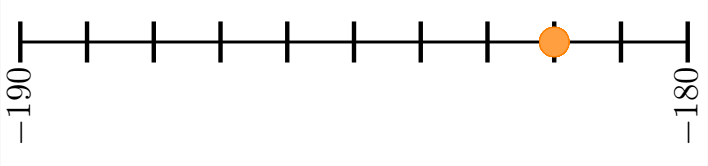
\includegraphics[width=150px]{../images/recta_num_-182.png} \\[-0.5em]   \fillin[$-182$][1.5in]
                  \part 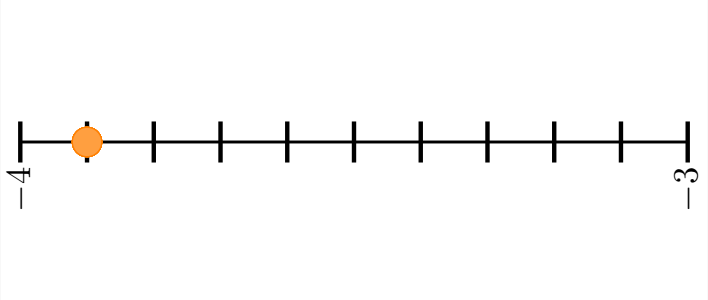
\includegraphics[width=150px]{../images/recta_num_-3.9.png} \\[-0.5em]  \fillin[$-3.9$][1.5in]
            \end{parts}
      \end{multicols}


      \subsection*{\ifprintanswers{Comparación de negativos}\else{}\fi}
      \question[4] Escribe sobre la línea el símbolo de mayor que ($>$), menor que ($<$), o igual ($=$) según corresponda.

      \begin{multicols}{2}
            \begin{parts}
                  \part $-182$ \fillin[$>$][0.5in] $-189$
                  \part $-97$ \fillin[$<$][0.5in] $-96.2$
            \end{parts}
      \end{multicols}

      \subsection*{\ifprintanswers{Suma y resta con negativos }\else{}\fi}
      \question[4] Realiza las siguientes sumas y restas con números negativos:

      \begin{multicols}{2}
            \begin{parts}
                  \part $-223+67=$ \fillin[$-156$][0in]
                  \part $(16)-(-14)=$ \fillin[$30$][0in]
            \end{parts}
      \end{multicols}

      \subsection*{\ifprintanswers{Multiplicación y división con negativos}\else{}\fi}
      \question[4] Realiza las siguientes multiplicaciones y divisiones con números negativos:
      \begin{multicols}{2}
            \begin{parts}
                  \part $(31)\divisionsymbol (-62)=$ \fillin[$-\dfrac{1}{2}$][0in]
                  \part $(-15)(-14)=$ \fillin[$210$][0in]
            \end{parts}
      \end{multicols}



      \subsection*{\ifprintanswers{Jerarquía de operaciones}\else{}\fi}
      \question[8] Usando la jerarquía de operaciones, realiza la siguiente operación

      \begin{multicols}{2}
            \begin{parts}
                  \part $9+6\times 4-5=$ \fillin[$28$][0in]
                  \begin{solutionbox}{2cm}
                        \[9+6\times 4-5=9+24-5=33-5=28\]
                  \end{solutionbox}

                  % \part $7+2^2 \times 6+2^2-6=$ \fillin[$29$][0in]
                  % \part $10\times 12-14\divisionsymbol 2+15=$ \fillin[$128$][0in]
                  % \part $6^3 \divisionsymbol 8 \divisionsymbol 9 = $ \fillin[$3$][0in]
                  \part $8\times 3 +70\divisionsymbol 7-7=$ \fillin[$27$][0in]
                  \begin{solutionbox}{2cm}
                        \[8\times 3 +70\divisionsymbol 7-7=24+10-7=34-7=27\]
                  \end{solutionbox}

                  % \part $16 \times 15 \divisionsymbol 5 +12=$ \fillin[$60$][0in]
            \end{parts}
      \end{multicols}

      \newpage
      \section*{\ifprintanswers{Sucesiones aritméticas}\else{}\fi}
      \subsection*{\ifprintanswers{Completando la sucesión}\else{}\fi}
      \question[4] Escribe los términos faltantes de las siguientes sucesiones aritméticas:
      \begin{multicols}{2}
            \begin{parts}
                  % \part $ -8,-13,-18,$\fillin[$-23$][0.3in], \fillin[$-28$][0.3in],\fillin[$-33$][0.3in],\ldots
                  \part $-57,-65,-73,$\fillin[$-81$][0.3in], \fillin[$-89$][0.3in], \fillin[$-97$][0.3in],\ldots
                  \part $-14,-17,-20,$\fillin[$-23$][0.3in], \fillin[$-26$][0.3in], \fillin[$-29$][0.3in],\ldots
                  % \part $-19,-15,-11,$\fillin[$-7$][0.3in], \fillin[$-3$][0.3in],\fillin[$1$][0.3in],\ldots
            \end{parts}
      \end{multicols}


      \subsection*{\ifprintanswers{Diferencia de una sucesión}\else{}\fi}
      \question[4] Determina la diferencia de las siguientes sucesiones aritméticas:
      \begin{multicols}{2}
            \begin{parts}
                  \part $-23,-15,-7,1,9,17,\ldots$ \fillin[$d=8$][0in]
                  % \part $-15,-10,-5,0,5,\ldots$ \fillin[$d=5$][0in]
                  % \part $-8,-13,-18,-23,-28,-33,\ldots$ \fillin[$d=-5$][0in]
                  % \part $-19,-15,-11,-7,-3,1,\ldots$ \fillin[$d=4$][0in]
                  % \part $7,9,11,13,15,17,\ldots$ \fillin[$d=2$][0in]
                  \part $-4,-2,0,2,4,6,\ldots$ \fillin[$d=2$][0in]
            \end{parts}
      \end{multicols}


      \subsection*{\ifprintanswers{Término general}\else{}\fi}
      \question[4] Determina el término general de las siguientes sucesiones aritméticas:
      \begin{multicols}{2}
            \begin{parts}
                  \part $3,9,15,21,27,\ldots$ \fillin[$6n-3$][1in]
                  % \part $-69,-72,-75,-78,-81,\ldots$ \fillin[$-3n-66$][1in]
                  % \part $40,35,30,25,20,\ldots$ \fillin[$5-5n$][1in]
                  % \part $-2,-6,-10,-14,-18,\ldots$ \fillin[$-4n+2$][1in]
                  % \part $-2,1,4,7,10,\ldots$ \fillin[$3n-5$][1in]
                  \part $-57,-65,-73,-81,-89,\ldots$ \fillin[$-8n-49$][1in]
            \end{parts}
      \end{multicols}


      \subsection*{\ifprintanswers{Término enésimo}\else{}\fi}
      \question[4] Encuentra el \textit{n-ésimo} término de la siguientes sucesiones aritméticas:
      \begin{multicols}{2}
            \begin{parts}
                  \part Calcula el término número 44 de la siguiente sucesión aritmética: $-3n-15$
                  \begin{solutionbox}{2cm}
                        \[-3(44)-15=-132-15=-147\]
                  \end{solutionbox}

                  \part Calcula el término número 47 de la siguiente sucesión aritmética: $-5,0,5,10,15,\ldots$
                  \begin{solutionbox}{2cm}
                        \[5(47)-5=235-5=225\]
                  \end{solutionbox}

                  % \part Calcula el término número 28 de la siguiente sucesión aritmética: $-69,-72,-75,-78,-81,\ldots$
                  % \begin{solutionbox}{2cm}
                  %       \[-3(28)-66=-84-66=-150\]
                  % \end{solutionbox}

                  % \part Calcula el término número 15 de la siguiente sucesión aritmetica: $11,18,25,32,39,\ldots$
                  % \begin{solutionbox}{2cm}
                  %       \[7(15)+4=105+4=109\]
                  % \end{solutionbox}

                  % \part Calcula el término número 25 de la siguiente sucesión aritmética: $2n-6$
                  % \begin{solutionbox}{2cm}
                  %       \[2(25)-6=50-6=44\]
                  % \end{solutionbox}

                  % \part Calcula el término número 22 de la siguiente sucesión aritmética: $7,2,-3,-8,-13,\ldots$
                  % \begin{solutionbox}{2cm}
                  %       \[-5(22)+12=-110+12=-98\]
                  % \end{solutionbox}
            \end{parts}
      \end{multicols}


      \subsection*{\ifprintanswers{Suma de una sucesión aritmética}\else{}\fi}
      \question[10] Calcula la suma de los primeros $n$ términos de las siguientes sucesiones aritméticas:
      \begin{multicols}{2}
            \begin{parts}
                  \part Calcula la suma de los primeros 41 términos de la siguiente sucesión aritmética: $40,51,62,73,84,\ldots$
                  \begin{solutionbox}{2.5cm}
                        \[a_{41}=40+11(41-1)=40+440=480\]
                        \[S_{41}=\dfrac{41(40+480)}{2}=10,660\]
                  \end{solutionbox}

                  \part Calcula la suma de los primeros 37 términos de la siguiente sucesión aritmética: $15,25,35,45,55,\ldots$
                  \begin{solutionbox}{2.5cm}
                        \[a_{37}=15+10(37-1)=15+360=375\]
                        \[S_{37}=\dfrac{37(15+375)}{2}=7,215\]
                  \end{solutionbox}

                  % \part Calcula la suma de los primeros 23 términos de la siguiente sucesión aritmética: $-5,0,5,10,15,\ldots$
                  % \begin{solutionbox}{2.5cm}
                  %       \[a_{23}=-5+5(23-1)=-5+110=105\]
                  %       \[S_{23}=\dfrac{23(-5+105)}{2}=1,150\]
                  % \end{solutionbox}

                  % \part Calcula la suma de los primeros 25 términos de la siguiente sucesión aritmética: $11,18,25,32,39,\ldots$
                  % \begin{solutionbox}{2.5cm}
                  %       \[a_{25}=11+7(25-1)=11+168=179\]
                  %       \[S_{25}=\dfrac{25(11+179)}{2}=2,375\]
                  % \end{solutionbox}
            \end{parts}
      \end{multicols}

\end{questions}
\end{document}